This chapter, is dedicated to the high-level design of the presented system. In this chapter we will explain the different concepts used in our policy engine. 

During our brainstorm sessions it quickly became clear that we needed a policy engine that was flexible. This we deducted from the cases discussed both amongst team members, but also based on several interviews with danish companies that were performed by a team member (see XXX?). With inspiration from other building management systems (see \nameref{chapter:relatedWork}) and looking at the web service we had to communicate with, we came up with the concept of policies that consist of to types of overall statements; \textit{if-statements} and \textit{set statements}. If-statements works as if-statements in many popular GPL's, with a condition consisting of expressions, a then-clause and an else-clause.

\section{The policy expression language}
Merriam-Webster defines \textit{policy} as; "A definite course or method of action selected from among alternatives and in light of given conditions to guide and determine present and future decisions."

We have defined a policy as a collection of conditional statements operating on sensors and actuators residing in the building simulator. The policy also has a start time and a stop time. It is also possible to de-activate a policy completely - without deleting it entirely.

A statement can either be a SetStatement or an IfStatement. The SetStatement sets an value in the simulator (in effect it is an actuator). The backend implementation allows nested If-statements, making the policies both flexible and simple (XXX how can we claim that?). An If-statement can contain multiple expressions that all are being anded when evaluated. If the user wants to make an If-statement with or'ed expressions, she will have to use a nested if. The optimal solution to this would have been to make a safe left-recursive model. We did not have enough time for this, but we will elaborate further on this subject in the discussion (XXX remember to elaborate). 

\section{Architecture}
The system that we have designed consists of four overall parts;
\begin{itemize}
	\item The management website (front end)
	\item The policy engine (back end)
	\item The database for storing policies (back end)
	\item The provided building simulator (back end)
\end{itemize}

Figure \ref{fig:design-system-architecture} illustrates the relationship of the system parts. In terms of MVC the \textit{model} and the \textit{controller} is the servlet containing data and business logic. The servlet reacts to several urls (see XXX), that functions as an interface for an operation needed in the system. The \textit{View} is the rendered html based on JQuery.

\begin{figure}[t]
\center{
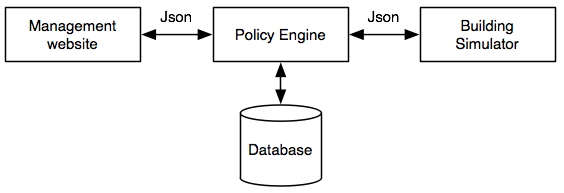
\includegraphics[scale=.5]{chapters/design-system-architecture.png}
\caption{The PolicyEngine system architecture.}\label{fig:design-system-architecture}}
\end{figure}

\subsection{The management website}
The management website resides is based in a small collection of html pages that relies heavily on JQuery. The building policy administrator opens the main page in a browser, and gets an overview of all the policies and can perform CRUD operations on them.

During the design phase for the GUI of the management website, we used Photoshop sketches that we mailed and transferred via Skype to each other. One from the kenyan team also assisted in this phase. After discussing how to best present policies to the building policy administrator in the time we had available, we choose an indented page layout when presenting the policies. By choosing this type of GUI, as opposed to a more tabular view on the if's, we elected a GUI that is flexible enough to extend to a recursive rendering which clearly matters a greatly when then-clauses can contain other if-statements that again contain then-clauses and so forth. For implementation see Section XXX.

\subsection{The policy engine}
The policy engine consists of a servlet and domain classes for the expression language needed to build policies. The servlet is the core of our policy engine. It has three main objectives;

\begin{figure}[b]
\center{
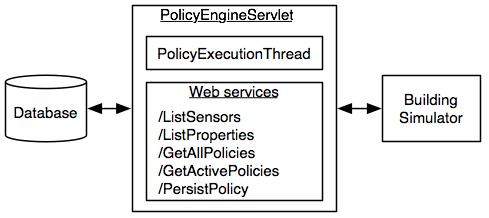
\includegraphics[scale=.5]{chapters/design-servlet-architecture.png}
\caption{A overview model of the PolicyEngineServlet.}\label{fig:design-servlet-architecture}}
\end{figure}

\begin{itemize}
	\item The timed, repetitive execution of policies that currently are active
	\item Serving web service requests to the JQuery front end
	\item Serving the management website html files
\end{itemize}

An overview model of the PolicyEngineServlet can be seen in Figure \ref{fig:design-servlet-architecture}.

As servlet container we use Tomcat 7.0.37. On servlet container startup the servlet will read various configuration values, and then set up a thread that manages the timed, repetitive execution of active policies. While testing the system policies were executed every 5 seconds, but this is configurable. The servlet will start by querying the database for active profiles, which are defined as policies that have a boolean flag (active) set to true, while the current time is within the policie's \textit{from} and \textit{to} time. This will result in a list of policies that should be executed. Then all sensor id values of all if-statements are fetched from the building simulator, and cached in an in-memory datastructure. Thereafter the policies are executed. 

This design was based on several iterations of group discussions. Everyone wanted a solution that worked efficient and fast, within the scope and timeframe that we initially had set for the system development. (XXX reference to project setup, project plan, scope, limitations?). 

The first couple of design proposals from some team members were based on SQL integration directly into the database that the building simulator uses. This direct integration could be argued as being a good, although strongly coupled integration. Also, it did not feel like a real world scenario (which we assume is one of the points of this course) if we could access the database directly in this way. Traditionally building systems tend to be closed source proprietary systems with few, if any, integration point (XXX reference to for example CTS systems).

Later design proposal revolved around the idea of having more or less mirrored sensor data in a separate database. Data should be transferred at regular intervals, and the policies should be executed against the copy. This turned out to be a too unsophisticated solution - and the problem to decide which sensor data remained. Finally we arrived at the rest api integration for fetching and setting values, and our own database to hold the policies and their time information.

\subsection{The database}
The database used is a mySQL 5.5.29 and used for storing the policies. At the moment we only use one table containing all the policies.

\subsection{The building simulator}
The building simulator provided in the course has not been changed or modified in any way.

\subsection{Limitations}

... Alternatives?